\section{Visi\'on}

\subsection{Introducci\'on}
Intro de visi\'on

\subsection{Trabajos previos}
	\subsubsection{Mobile Field Robot with Vision-Based Detection of Volunteer Potato Plants in a Corn Crop - FRITS K. VAN EVERT}
	\cite{potato}
	\subsubsection{Review of shape representation and description techinques - Dengsheng Zhang}
El objetivo de este trabajo es realizar un resumen de las tecnicas mas importantes en cuanto a la representación y descripción de formas.
	\subsubsection{Sidewalk Following Using Color Histograms - John S. Seng}
	\subsubsection{Skin Detection using HSV color space - V. A. Oliveira, A. Conci}
	En este artículo se trabajó sobre la detección de piel en imágenes utilizando el espacio de color HSV. El algoritmo propuesto 
por el autor consiste en el filtrado de los pixels en base al valor del canal de tonalidad ( canal H ). Los rangos de valores utilizados para 
representar el color de la piel fueron obtenidos de otros articulos relacionados. Luego, con el objetivo de eliminar ruido, se aplican filtros morfologicos y de suavizado, estos son (en este orden) dilatación, erosión y un filtro de mediana. Para los filtros morfologicos se utilizaron nucleos de 5x5 pixels mientras que para el filtro de mediana se usaron nucleos de 3x3 pixels. Finalmente, el autor midió la performance de su algoritmo utilizando imágenes de prueba en donde se aprecian distintas zonas con piel aisladas. A partir de estas imagenes, se obtuvieron las coordenadas de los pixels que se corresponden con piel y se las contrastó con aquellas que identificó el algoritmo. Los resultados presentados para 4 imágenes son satisfactorios obteniendo en promedio un porcentaje de falsos negativos cercano al 1\% y de falsos positivos menor al 6\%.

	\subsubsection{Line Detection and Lane Following for an Autonomous Mobile Robot - Andrew Reed Bacha}
	En este artículo se describió el software utilizado para uno de los robots ganadores de la competencia "Intelligent Ground Vehicle Competition" (IGVC) en donde se requiere que los robots naveguen  a traves de un camino delimitado por lineas pintadas sobre cesped en un ambiente al aire libre en donde se pueden presentar obstáculos. El robot utilizaba una única cámara para el sistema de visión y su objetivo era detectar las lineas pintadas 
para determinar la dirección de movimiento del robot. El algoritmo descripto por el autor cuenta con una etapa de pre-procesamiento y otra de detección de lineas. En la etapa de pre-procesamiento se comienza por convertir la imágen a escala de grises utilizando una transformación en la que la intensidad de cada pixel es determinada usando $2*B(i,j) - G(i,j)$ con el argumento que el canal verde contiene ruido provocado por la exposición de luz en el pasto y de esta mánera se lo elimina. Luego el autor propone utilizar un ajuste de brillo argumentando que los pixels de la zona mas alta se encuentran mas expuestos a la luz por la perspectiva de la camara, para esto sustrae una máscara que compensa este efecto. Además, el autor elimina la proyección del robot mismo sobre la cámara. En la etapa de detección se procedió realizando un threshold para obtener los pixels mas brillantes. Luego, la salida del threshold se utilizó como entrada para un detector de lineas basado en el algoritmo de hough. Finalmente, según la orientación de las lineas detectadas se determina la dirección del robot. El algoritmo se consideró exitoso ya que el robot propuesto fue el ganador de la competencia.


	
\subsection{Algoritmo de detección}
\subsubsection{Estructura}
La figura \ref{fig:alg_steps} ilustra las etapas del algoritmo. Este fue programado utilizando el lenguaje C++ y la librería de visión computacional openCv.
El algoritmo comienza por tomar una imágen fresca de la cámara, las imágenes capturadas poseen el formato 24-bit RGB. A su vez, esta imagen puede ser descompuesta en 3 imágenes o canales de 8 bits , una para cada color ( rojo ,verde y azul). Con el objetivo de minimizar el impacto producido por cambios en la iluminación se convierte la imagen al formato HSV (tono, saturación y brillo). Luego utilizamos el canal H de esta nueva imágen para establecer que pixels se corresponden con el color buscado, filtrando aquellos pixeles que no coinciden con el rango deseado. A su vez, usamos la información brindada por los  canales de saturación y/o brillo para obtener mas precisión sobre el color de los pixeles.\\
	\indent Descartamos los pixels filtrados en el canal de saturación realizando un and bit a bit con la imagen filtrada.  En la siguiente etapa, se utilizan filtros morfológicos cuyo objetivo es la eliminación de ruido. El resultado de aplicar estos filtros resulta en la expansión de las areas donde hay mucha presencia de pixeles de interés, produciendo un área de intensidad homogénea mientras que elimina la aparición aislada de estos producto del ruido. El paso siguiente consiste en la aplicación de un umbral. El umbral filtra aquellos pixeles que no se encuentren por encima de un valor mínimo de intensidad marcandolos con valor cero y conserva únicamente los pixeles que si lo hacen estableciendoles un valor predeterminado ( mayor a cero). \\
	\indent Hasta aquí el pre-procesamiento de la imágen, al llegar a esta etapa del algoritmo deseamos tener solo pixeles de los potenciales objetos de interés. Vale notar que, como consecuencia de aplicar un filtro umbral, la imagen se encuentra binarizada, es decir, los pixels solo pueden tener dos posibles valores: cero (negro) si no es un pixel de interés o mayor a cero en el caso contrario. Es entonces que automáticamente quedan delimitadas las áreas que contienen pixeles de interés, el próximo paso del algoritmo se encarga de obtener los contornos de estas áreas. Para esto utilizamos el algoritmo de suzuki \cite{suzuki85} que recorre los bordes de estas zonas y crea secuencias de puntos $(x,y)$ que definen el contorno de las mismas. Las secuencias de puntos son luego aproximadas para generar polígonos cerrados mediante el algoritmo de Douglas-Pecker \cite{dp74}. Tomando estos polígonos definimos distintos parámetros tales como el área, perimetro o figura que nos permiten discernir si se trata de un objeto a reconocer o no.


\begin{figure}[tpb]
\begin{center}
  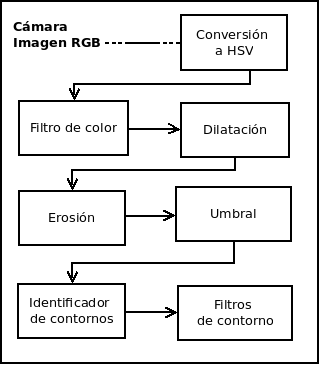
\includegraphics[scale=0.6]{figuras/vision-flow.png}
\end{center}
  \caption{Etapas del algoritmo de visión }
  \label{fig:alg_steps}
\end{figure}


\subsubsection{Detecci\'on de color}
El problema de decidir si un pixel determinado se corresponde con un color particular resulta mucho mas sencillo de resolver en el espacio de color HSV. En el espacio RGB, de haber un cambio en el brillo o iluminación de la imagen, los tres canales se ven afectados de igual manera mientras que en el espacio HSV el canal H, que codifica la información sobre el tono del color, se ve mucho menos influenciado que los otros dos canales ( saturación y valor). De esta manera, podemos caracterizar el color de un pixel determinado observando su valor en dicho canal sin importar las condiciones de brillo o iluminación al cual se encuentra expuesto.
\\ \indent Entonces, realizamos la detección de color verificando los valores correspondientes al canal H ( tono) de la representación HSV de la imagen. Para esto realizamos la conversión de la imagen obtenida por la cámara  de formato RGB a HSV usando el algoritmo expuesto en la figura \ref{code:hsv}.
\begin{figure}[tpb]
\begin{verbatim}
V=max(R,G,B)
S=(V-min(R,G,B))*255/V   if V!=0, 0 otherwise

       (G - B)*60/S,  if V=R
H= 180+(B - R)*60/S,  if V=G
   240+(R - G)*60/S,  if V=B

if H<0 then H=H+360
\end{verbatim}
\label{code:hsv}
\caption{pseudo-código de la conversión RGB-HSV}
\end{figure}

Obteniendo el canal H, nos fijamos que los valores de los pixeles esten dentro de cierto rango correspondiente al color que buscamos. Como podemos observar en la figura \ref{fig:hsv_space} En el espacio de color HSV los colores se encuentran dispuestos a lo largo de una circunferencia , donde cada tonalidad representa un ángulo en la misma. Por ejemplo, si queremos abarcar las distintas tonalidades del azul podemos elegir el rango que va de 200$^\circ$ a 260$^\circ$. Cuando buscamos un color en particular  es preciso elegir este rango cuidadosamente ya que de ser un rango muy restrictivo podemos despreciar pixeles de interés arruinando la forma del contorno del objeto a buscar y si elegimos un rango más abarcativo podemos tomar pixeles de colores distintos al buscado, introduciendo ruido en las formas de los contornos. Experimentalmente se comprueban los resultados de un filtro de color con distintos rangos, como se muestra  en la figura \ref{fig:hue_range}.
\begin{figure}[tpb]
\begin{center}
  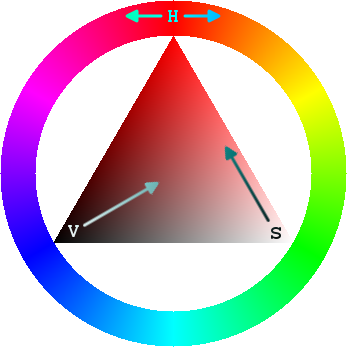
\includegraphics[scale=0.4]{figuras/hsv_triangle.png}
\end{center}
  \caption{\small Espacio de color HSV. Los distintos tonos de colores se encuentran dispuestos a lo largo de la circunferencia.}
  \label{fig:hsv_space}
\end{figure}

\begin{figure}[tpb]
\begin{center}
  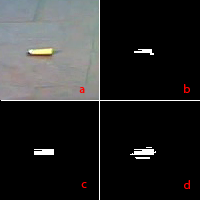
\includegraphics[scale=0.8]{figuras/hue.png}
\end{center}
  \caption{\small Resultados de aplicar un filtro de color utilizando distintos rangos. (a) Captura original . (b) Resultado de aplicar el filtro $35\le h \le45$, se pierden algunos pixeles. (c) Resultado de aplicar el filtro $20\le h \le40$. (d) Resultado de aplicar el filtro $10 \le h \le 50$, se introducen pixeles extra.} 
  \label{fig:hue_range}
\end{figure}

	\subsubsection{Threshold}
Threshold o umbral es una operación que nos permite pasar de una imagen en escala de grises a una imagen binaria. El proceso de thresholding consiste en distinguir los pixeles que se encuentran por encima de un cierto valor de los que estan por debajo del mismo. Con este objetivo, se crea una imagen binaria asignandoles valores 1 o 0 según su condición respecto del valor. El algortmo de thresholding nos puede servir para distinguir un objeto determinado de un contexto o fondo siempre y cuando el objeto posea un mayor brillo que el fondo en el que se encuentra. Esto significa que los pixeles correspondientes a un objeto se encontrarán por encima de cierto valor caracteristico, determinado por el fondo. En nuestro caso esto no sucede de esta forma ya que no siempre la intesidad / brillo de los objetos supera al fondo en el que se encuentra, por lo cual resulta difícil utilizar esta técnica. Podemos apreciar un ejemplo de este efecto en la figura \ref{fig:thresh-dif}. \\
\indent Existen diversas variantes de threshold, los parametros utilizados son $V$ para indicar el valor umbral y $M$ que indica el valor a setear en los pixeles.
\begin{itemize}
\item{ Threshold binario:  Si un pixel se encuentra por encima de $V$, se le asigna un valor $M$, de otro modo se le asigna $0$.}
\item{ Threshold binario invertido:  Si un pixel se encuentra por encima de $V$, se le asigna 0, de otro modo se le asigna $M$.}
\item{ Threshold truncado:  Si un pixel se encuentra por encima de $V$, se le asigna $V$, de otro modo conserva su valor.}
\item{ Threshold a cero invertido : Si un pixel se encuentra por encima de $V$ se le asigna $0$, de otro modo, conserva su valor.}
\item{ Threshold a cero invertido : Si un pixel se encuentra por encima de $V$ conserva su valor, de otro modo se lee asigna $0$.}
\end{itemize}
El problema con esta familia de algoritmos es que en todos los casos el valor $V$ permanece constante para toda la imagen haciendolo propenso a errores cuando la imagen presenta diferentes niveles de iluminación. Una manera de solucionar esto es pre-computando el valor $V$ para distintas zonas de la imágen. Un ejemplo de esta solución es la técnica de thresholding adaptativo, que computa el valor de $V$ a medida que recorre la imagen, usando para esto, una ventana cuyo tamaño es definido por el usuario. Siguiendo esta lógica, se utilizan los valores de los pixeles locales a esta ventana para definir un valor de $V$ (por ejemplo calculando el promedio de intensidad) y luego se aplica alguna de las técnicas de thresholding simples mencionadas, utilizando este mismo valor. Sin embargo, este algoritmo es mas costoso y puede provocar efectos indeseados.ACA PODRIA IR UNA FOTO DE THRESHOLD ADAPTATIVO\\
\indent En nuestro caso, utilizamos thresholding no para distinguir los objetos del fondo ( esto es trábajo del filtro de color), sino como metodo de eliminación de ruido. Cuando se combina el canal de saturación con el resultado del filtro de color, se obtiene una imagen de escala de grises que esta segmentada en un conjunto de areas con distintos valores de intensidad. Luego de aplicar dilatación y erosión, los niveles de intensidad de cada área se vuelven homogeneos ( ya que se toma el máximo o mínimo local) y es entonces donde podemos diferenciar las zonas de intensidad alta de las zonas de intensidad baja, motivo por el cual utilizamos la operación de threshold. COMPLETAR AQUI \ref{fig:threshold_ruido} \ref{fig:threshold}. 
\begin{figure}[tpb]
\begin{center}
  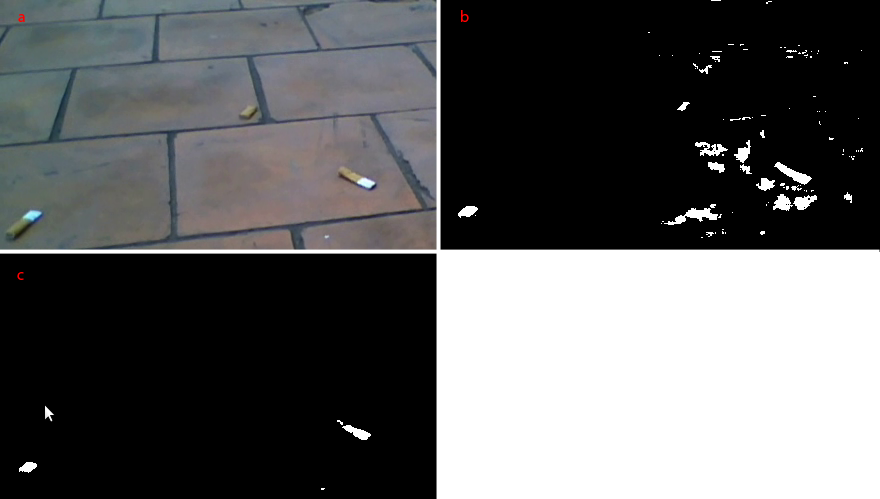
\includegraphics[scale=0.4]{figuras/threshold-dif.png}
\end{center}
  \caption{\small Distintos valores de umbral. (a) Captura original. 
  (b) Threshold binario con umbral 120. Se observan pixeles extra en 
  la detección. (c) Threshold binario con umbral 160. Se observa la 
  ausencia de pixeles. }
  \label{fig:thresh-dif}
\end{figure}


\begin{figure}[tpb]
\begin{center}
  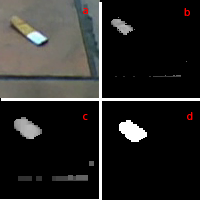
\includegraphics[scale=0.8]{figuras/threshold-ruido.png}
\end{center}
 \caption{\small Resultados de aplicar thresholding binario. (a) Captura original . (b) Salida del detector de color, se observan algunos pixeles extra cerca de la línea de brea. (c) Salida de la operación de dilatación-erosión. (d) Salida de la operación de thresholding binario con un umbral de $100$. La baja intensidad de los pixeles extra en la línea de brea no supera el umbral propuesto y por lo tanto son descartados. El contorno del objeto de interés se conserva aislado.} 
  \label{fig:threshold_ruido}
\end{figure}

\begin{figure}[tpb]
\begin{center}
  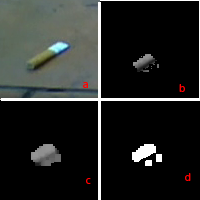
\includegraphics[scale=0.8]{figuras/threshold.png}
\end{center}
  \caption{\small Resultados de aplicar thresholding. (a) Captura original . (b) Salida del detector de color, se observan algunos pixeles extra debajo del objeto de interés. (c) Salida de la operación de dilatación-erosión, los pixeles extra se combinaron con los pixeles del objeto.(d) Salida de la operación de thresholding binario con un umbral de $100$. La baja intensidad de los pixeles extra en la zona debajo del objeto no supera el umbral propuesto y por lo tanto son descartados. El contorno del objeto de interés se conserva aislado.} 
  \label{fig:threshold}
\end{figure}

	\subsubsection{Operaciones morfológicas}
Sombras, luces y otros efectos pueden alterar el resultado del filtro de color introduciendo ruido en los objetos a detectar. Este ruido puede surgir tanto de la omisión de pixeles de interés como por la inclusión de pixeles extra. Para subsanar esto, utilizamos las operaciones morfológicas de dilatación y erosión. Ambas se basan en la utilización de un elemento estructural, esto es, una figura de cualquier tamaño y forma que tiene definido un punto principal y que recorre la imágen solapandose pixel a pixel. De acuerdo a operaciones locales a este elemento, el pixel que coincide con el punto principal se ve modificado. Usualmente se utilizan como elementos estructurales , pequeños discos o cuadrados, donde el punto principal se encuentra en el centro del mismo. El efecto generado se entiende mejor observandolo en imágenes binarias. En el caso de la dilatación, la idea intuitiva es remplazar cada pixel no vacío con una copia del elemento estructural cuyo punto principal se encuentra en esa posición. Para la erosión, la idea intuitiva es quedarse con aquellos pixeles tal que podamos hacer caber un elemento estructural cuyo punto principal se encuentra en esa posición y dicho elemento solo cubra pixeles no vacíos.
Ilustramos esto en las figuras \ref{fig:erode-sample} y \ref{fig:dilate-sample}.


\begin{figure}[tpb]
\begin{center}
  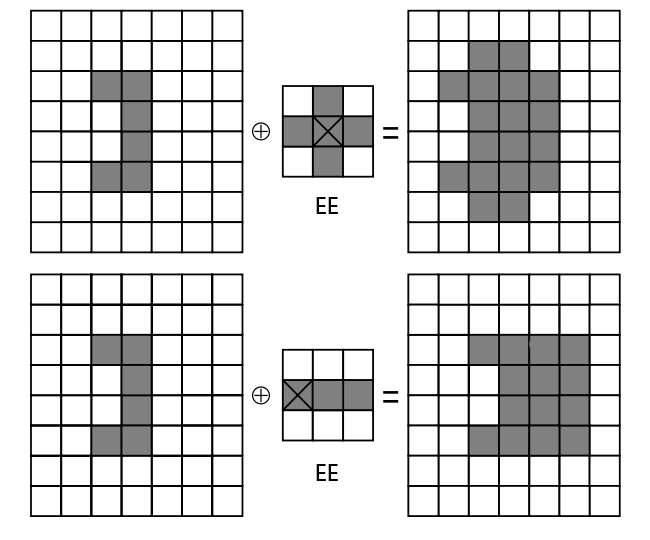
\includegraphics[scale=0.4]{figuras/dilate-sample.png}
\end{center}
  \caption{\small Operación de dilatación en imágenes binarias. Se reemplazan los pixeles no vacíos por una copia del elemento estructural con punto principal en esa posición. La cruz indica la posición del punto principal dentro del elemento estructural (ee). Imagen obtenida del curso de visión artificial de la Universidad Politécnica de Madrid.}
  \label{fig:dilate-sample}
\end{figure}

\begin{figure}[tpb]
\begin{center}
  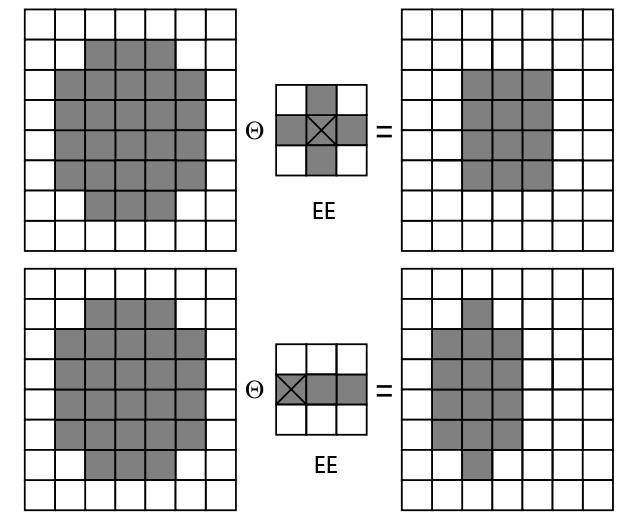
\includegraphics[scale=0.4]{figuras/erode-sample.png}
\end{center}Podemos apreciar un ejemplo de threshold en la figura \ref{fig:threshold}
  \caption{\small Operación de erosión en imágenes binarias. Se persisten los pixeles no vacíos en donde cabe una copia del elemento estructural cuyo punto principal se encuentra en esa posición. La cruz indica la posición del punto principal dentro del elemento estructural (ee). Imagen obtenida del curso de visión artificial de la Universidad Politécnica de Madrid. } 
  \label{fig:erode-sample}
\end{figure}

	\subsubsection*{Dilataci\'on}
En imágenes no binarias, la operación de dilatación se define tomando el máximo local bajo el elemento estructural y poniendole ese valor al punto principal. El efecto producido es una reducción general en el brillo de la imagen y un probable aumento el tamaño de las fíguras \cite{nasa-dilate-erode}.  Cuando un área grande aparece, a causa del ruido, partida en varias componentes, el uso de la operación de dilatación provoca que  se combinen nuevamente en una sola. Un ejemplo de esto puede ser apreciado en la figura \ref{fig:dilate}. Otro beneficio de utilizar dilatación es la eliminación del ruido espurio como se aprecia en la figura \ref{fig:dilate-ruido}.

\begin{figure}[tpb]
\begin{center}
  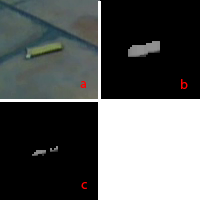
\includegraphics[scale=0.8]{figuras/dilate1.png}
\end{center}
  \caption{\small Efecto de la operación de dilatación. (a)  Imagen original tomada de la cámara. (b) Imágen luego de aplicar dilatación a la imagen c con un elemento estuctural cuadrado de 3x3 pixels, con punto principal en el centro. (c) Salida del filtro de color combinado con el canal de saturación. La colilla de cigarrillo esta 'partida' en dos componentes conexas. } 
  \label{fig:dilate}
\end{figure}

\begin{figure}[tpb]
\begin{center}

  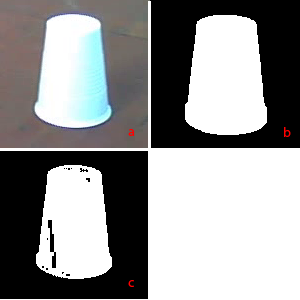
\includegraphics[scale=0.6]{figuras/dilate-ruido.png}
\end{center}
  \caption{\small Eliminación de ruido mediante la operación de dilatación. (a) Imagen original tomada de la cámara. (b) Imágen luego de aplicar dilatación a la imagen c con un elemento estuctural cuadrado de 3x3 pixels, con punto principal en el centro. (c) Salida del filtro de color. Observamos áreas  oscuras en el interior del vaso. }
  \label{fig:dilate-ruido}
\end{figure}

	\subsubsection*{Erosi\'on}
En imágenes no binarias, la operación de erosión se define tomando el mínimo local bajo el elemento estructural y poniendole ese valor al punto principal. Contrario a la dilatación, este operador generalmente reduce el brillo de la imagen y disminuye el tamaño de las figuras \cite{nasa-dilate-erode}. Usamos la operación de erosión para eliminar las protuberancias que pueden surgir de aplicar la operación de dilatación. En la figura \ref{fig:erode} podemos apreciar el efecto de aplicar dilatación y luego erosión.

\begin{figure}[tpb]
\begin{center}
  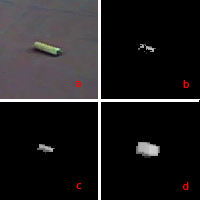
\includegraphics[scale=0.8]{figuras/erosion.png}
\end{center}
  \caption{\small Ejemplo de erosión. (a) Captura original. (b) Salida del filtro de color. Se observan fallas en la detección del objeto. (d) Se aplica la operación de dilatación a la imagen b. Se observa la producción de protuberancias en la figura del objeto. (c) Salida luego de aplicar erosión a c. La figura del objeto se corrige eliminando parte de las protuberancias. Sin embargo, no se observan fallas en la detección del objeto. }
  \label{fig:erode}
\end{figure}

	\subsubsection{Detecci\'on de contornos}
		\subsubsection*{Algoritmo}
		\subsubsection*{Representaci\'on}
	\subsubsection{Filtros}
	\subsection{Sistema de predicci\'on}
	El algoritmo de visión que hemos descripto hasta aquí funciona 
	procesando la imagen correspondiente a un único cuadro. Sin embargo, 
	el sistema de visión del robot debe permitir el reconocimiento de 
	objetos a medida que esta se desplaza por su entorno y por lo tanto 
	dicho sistema debe procesar imágenes secuenciales del mismo. Con 
	esto queremos decir que existe cierta relación entre las imágenes 
	que el sistema de visión debe procesar y que podemos aprovechar esta 
	caracteristica para reforzar la detección de objetos.  El mecanismo por el cual buscamos lograr este objetivo es el del sistema de predicción.\\
\indent 	El sistema de predicción consume la información que el 
sistema de visión le entrega en cada cuadro y, con ella, realiza el 
seguimiento de objetos a lo largo del tiempo. Es a partir de este 
seguimiento que el sistema de predicción toma decisiones sobre la 
posición o existencia de los objetos que el sistema de visión 
reconoce. Vale destacar que estos dos sistemas pueden encontrarse, a 
menudo, en desacuerdo acerca de la ubicación o de la misma existencia 
de un objeto.  El sistema de predicción se basa en las siguientes asumpciones:
\begin{enumerate}
\item{ Los objetos no realizaran grandes desplazamientos entre cuadros contiguos - esto se debe la proximidad temporal entre cuadros y que el robot no realiza movimientos bruscos.}
\item{ Los objetos no sufriran grandes alteraciones en su forma, área o perímetro entre cuadros contiguos - con un razonamiento similar, la perspectiva no cambia lo suficiente como par alterar la figura,área o perimetro de los objetos.}
\end{enumerate} 
Con estas premisas, dado un objeto $A$ reconocido en el cuadro $c_0$, 
cuyo centroide se encuentra en las coordeandas (en la imagen) $(x_0,y_0)$, área $a$ y perimetro $p$, 
el sistema de predicción asume que si se encuentra un objeto $A'$ en 
el cuadro siguiente $c_1$ con coordeandas $(x_1, y_1)$ tal que 
$||(x_1,y_1) - (x_0,y_0)||\leq \alpha$, área $a'$ tal que $|a-a'| \leq 
\gamma *a$ y perímetro $p'$ tal que $|p-p'|\leq \theta*p$ entonces $A 
\simeq A'$, donde $\alpha$ , $\gamma$ y $\theta$ son parametros del 
sistema. Esta aseveración no solo vale para el cuadro subsiguiente 
$c_1$ sino también para los siguientes $c_2,c_3 ... c_{0+\eta}$ donde 
$\eta$,$\alpha$ y $\gamma$ se computan, para este caso, según el 
historial de detección de cada objeto.  Con esta proposición, el 
sistema de predicción estima la posición de los objetos en el caso de 
que el sistema de visión no los reconozca. Con este fin, cuando un objeto es detectado a lo largo de varios cuadros se persiste la siguiente información:
\begin{itemize}
\item{ Última posición,área y perímetro - Se toman los datos de la detección mas reciente del sistema de visión .}
\item{ Antiguedad del objeto - Cantidad de cuadros transcurridos desde que se comenzo a persistir el objeto en el sistema de predicción.}
\item{ Cantidad de detecciones - Se mantiene la cantidad de cuadros en la cual el sistema de visión detectó al objeto.}
\item{ Desplazamiento en la posición - Si el objeto es detectado más 
de una vez, se almacena el desplazamiento en la posición $(x_1 - x_0 , y_1 - y_0 )$.}
\item{ Antiguedad de la última detección - Cantidad de cuadros que transcurrieron desde la última detección por parte del sistema de visión.}  
\end{itemize}
Esta información no solo nos permite corregir al sistema de visión 
cuando este no detecta un objeto sino que también podemos corregirlo 
cuando este detecta objetos de manera falsa, es decir, que no se 
encuentran en la posición informada o no existen del todo. Para 
implementar estos mecanismos se establecen las siguientes reglas sobre 
la persistencia de objetos:
\begin{enumerate}
\item{Un objeto debe ser detectado por el sistema de visión en $\delta$ 
cuadros consecutivos para ser considerado como tal por el sistema de 
predicción}
\item{El sistema de predicción descarta un objeto considerado si el 
sistema de visión no lo detecta en un número $\eta$ de cuadros 
consecutivos.}
\item{ $\eta$ se calcula cada $\lambda$ cuadros como 
$\frac{antiguedad}{detecciones}*\rho$ donde $\rho$ es un parametro del 
sistema}.
\item{ Si un objeto es considerado por el sistema de predicción y este 
no es detectado por el sistema de visión para algún cuadro entonces 
el sistema de visión realiza una estimación de su posición de 
acuerdo a la información obtenida de cuadros anteriores.}
\end{enumerate}

Estas reglas, aunque parezcan complejas por el número de variables que 
manejan, son realmente intuitivas. El sistema de predicción consume la 
información que el sistema de visión le brinda y la manipula con 
cierta desconfianza de acuerdo a su 
conveniencia. En una primera instancia, los objetos deben ganarse la 
confianza del sistema de predicción apareciendo regularmente en 
cuadros contiguos, esto esta vinculado a la asumpción número 
1. Por este motivo, utilizamos la regla 1 para eliminar aquellos objetos que 
no cumplen dicha suposición. \\
	Habiendose ganado la confianza del sistema de predicción, este 
	último comienza a tener a estos objetos en consideración y veta por su 
existencia aunque el sistema de visión no los detecte. El grado en que 
el sistema cree en la existencia de estos objetos se va regulando de 
acuerdo al historial de apariciones de los mismos. Si estos abusan de 
la confianza otorgada entonces el sistema de predicción los descarta 
como indica la regla 2. 
Este grado de confianza o de libertad se traduce en cantidad de 
cuadros que puede pasar un objeto sin ser detectado por el sistema de 
visión y siendo considerado por el sistema de predicción. Dicho 
número se determina periodicamente utilizando la fórmula de la regla 3.
Finalmente, durante este lapso de confianza, el sistema de predicción 
'adivina' la posición de los objetos si estos no son detectados por el 
sistema de visión, como dice la regla 4. \\
\indent La variable $\alpha$ determina la distancia máxima que puede 
desplazarse un objeto entre cuadros para que el sistema de predicción lo considere 
como el mismo. Las variables $\gamma$ y $\theta$ determinan el máximo 
porcentaje de variación en el área y perímetro que puede soportar un 
objeto entre cuadros para ser considerado como el mismo. Valores 
tipicos para la detección de colillas y vasos son de 
$0.1\leq\gamma\leq0.3$ y $0.1\leq\theta\leq0.3$. Para el caso de 
$\alpha$ definimos un valor aproximado de 30 pixeles. Sin embargo, la 
tolerancia en el desplazamiento varía según los cuadros transcurridos desde la última 
detección. Si en el cuado anterior fue detectado entonces se utiliza 
$\alpha$ , si fue detectado hace dos cuadros entonces $2*\alpha$,3 
cuadros $3*\alpha$ y así. La variable $\delta$ establece el úmbral de 
detección de un objeto por parte del sistema de visión para que el 
sistema de predicción lo empieze  a considerar. Para la detección de 
colillas se establecieron tres cuadros de úmbral mientras que para los 
vasos 2 cuadros. $\rho$ estable , independientemente de su 
regularidad, la cantidad máxima de cuadros que puede permanecer un 
objeto sin ser detectado y mantenido por el sistema de predicción. En 
ambos casos (colillas y vasos) establecimos 10 cuadros.\\ 
\indent Es importante destacar que tanto $\rho$ como $\delta$ repercuten directamente en la 
performance de detección. En el caso de la variable $\delta$, el 
sistema de visión debe reconocer un objeto $\delta -1$ veces antes de que sea 
tenido en cuenta por el sistema de predicción y, en este lapso, las 
detecciones seran ignoradas. Sin embargo, las apariciones no sostenidas 
(de hasta $\delta -1$ cuadros) de elementos que aparentan ser objetos 
para el sistema de visión pero no lo son, son también ignoradas, 
disminuyendo el porcentaje de falsos negativos.\\
\indent La variable $\rho$, en cambio, establece otro tipo de balance. 
	Siempre que un objeto deja de aparecer en la imagen (por 
	desplazamiento del objeto o del robot), el sistema de 
	predicción arriesga la posición de este un máximo de $\rho$ veces 
	(según la regularidad de detección) y, en esta caso, las equivoca a 
	todas ya que el objeto cesó de figurar en la imágen. El lado 
	positivo es que cuando un objeto que tenía un historial de 
	detección positivo es ocluido o alterado de tal forma que el 
	sistema de visión no lo reconoce, el sistema de predicción 
	arriesgará la posición (hasta $\rho$ veces) pudiendole acertar o no hasta que el objeto 
	sea nuevamente detectado por el sistema de visión o sea descartado. 
	Es en esta última situacion donde se obtienen nuevas detecciones que el sistema de visión 
	nunca podría obtener por si solo.\\
	\indent A partir de estas reflexiones surge la importancia de configurar 
	estas variables de acuerdo al sistema de visión que estemos 
	usando. Si tenemos un sistema de visión con alto porcentaje de 
	falsos positivos y bajo porcentaje de falsos negativos entonces es 
	probable que arriesgar más posiciones de objetos cuando estos no 
	son detectados mejore la performance. En este caso debemos elegir 
	valores de $\rho$,no muy pequeños, para afrontar el deficit de 
	detección del sistema de visión  y valores de $delta$,mas bien 
	pequeños, para no entorpecer la detección. Es importante remarcar 
	que el bajo porcentaje de falsos positivos, en este caso, nos 
	permite confiar en el sistema de visión en el sentido de que las cosas que 
	este detecte tienen altas probabilidades de ser objetos. \\
	\indent En el caso reciproco, un sistema de visión con alto 
	porcentaje de falsos negativos y bajo porcentaje de falsos 
	positivos quizas convenga tener un valor de $\delta$ alto, para 
	filtrar la mayor cantidad de detecciones falsas. Al hacerlo, puede 
	suceder que también filtremos detecciones positivas pero en ese 
	caso habría que estudiar cuanto se gana y cuanto se pierde y 
	buscar un balance.\\
	\indent Otra posibilidad es que el sistema de visión sea muy 
	confiable ( bajo porcentaje de falsos positivos/negativos). En 
	esta situación conviene configurar al sistema de predicción para 
	que haga más caso de lo que el sistema de visión le informa. Esto 
	significa que cuando el sistema de visión no encuentra un objeto 
	el sistema de predicción no debe arriesgar mucho ya que el objeto 
	probablemente no se encuentre. Asimismo, unas pocas detecciones de 
	un objeto bastan para que el sistema de predicción lo tenga 
	en cuenta  ya que hay una alta probabilidad de que 
	realmente se trate de un objeto. Esto se traduce en valores de 
	$\delta$ y $\rho$ bajos.
 


  %~ La regla 1 nos permite eliminar las detecciones 
%~ espontáneas de objetos por parte del sistema de visión. Si observamos nuevamente la 
%~ asumpción número 1, entonces no esta mal decir que un objeto que 
%~ fue detectado en un cuadro determinado debería aparecer(con cierta 
%~ probabilidad) en los subsiguientes. Bajo 
%~ este criterio utilizamos la regla 1 para descartar a aquellos objetos 
%~ que no cumplen con dicha proposición. En cambio, si el objeto es detectado de forma 
%~ regular en un número de cuadros estipulados, entonces el sistema de 
%~ predicción da fé de la existencia de ese objeto otorgandole la 
%~ posibilidad de no ser detectado por el sistema de visión por un 
%~ número determinado de cuadros. En este caso, el sistema de predicción 
%~ veta por la existencia del objeto ya que dispone de una muestra 
%~ suficiente para creer eso.  Esta creencia se mantiene por un número de 
%~ cuadros que se calcula de acuerdo al grado de regularidad en el que fue 
%~ detectado anteriormente. Para ejemplificar, un objeto que aparecio en 10 de los últimos 12 
%~ cuadros podrá permanecer mas cuadros sin ser detectado por el sistema 
%~ de visión y, sin ser descartado por el de predicción, que otro objeto 
%~ que solo apareció en 5 de los últimos 12 cuadros. Cuando se agota la 
%~ cantidad de cuadros que un objeto puede no ser detectado, el sistema 
%~ de predicción lo descarta. 
%~ . 

	\subsection{Focalización}
	Focalización es el mecanismo que busca que el sistema de visión se concentre en la detección de un único objeto a lo largo del tiempo. Esta situación es deseable cuando el sistema de visión ya detectó una basura y el robot se dirige a recolectarla. En esta circunstancia, no nos interesan otros objetos que puedan aparecer durante el trayecto y por lo tanto tratamos de evitar cualquier tipo de procesamiento innecesario sobre ellos. Con este objetivo, seleccionamos una sub-imagen a procesar en la cual suponemos que vamos a encontrar al objeto en cuestión. El mecanismo de focalización se encuentra muy ligado al sistema de predicción ya que debe persistir cierta información sobre un objeto a lo largo del tiempo.\\
\indent El mecanismo de focalización puede separarse en dos etapas. En una primera etapa, utlizando la información brindada por el sistema de predicción, se selecciona un objeto a focalizar. Existen varios criterios de selección, algunos que consideramos mas relevantes son:
\begin{itemize}
\item{ Objeto mas cercano - Se estiman las distancias a los objetos y se selecciona aquel que se encuentre mas cercano al robot.}
\item{ Objeto más detectado en los últimos 20 cuadros - Se selecciona al objeto que fue reconocido mas veces por el sistema de visión en las últimas 20 imágenes.}
\item{ Objeto más antiguo - Se elige al objeto que persistió más cuadros según el sistema de predicción.}
\item{ Combinación ponderada - Se utilizan los  criterios mencionados dandoles mayor o menor peso a cada uno y eligiendo al objeto que obtenga mayor puntuación.}
\end{itemize}
Pensamos todos los criterios con el objetivo de maximizar las chances de que el robot tenga exito en la recolección del objeto. El criterio de menor distancia implica un menor recorrido hacia el objeto y por lo tanto menos posibilidades de cometer error durante el recorrido. Si utilizamos el criterio de mayor detección en los últimos 20 cuadros estamos maximizando las chances de que el sistema de visión detecte al objeto durante el trayecto del robót hacia el mismo. Con un razonamiento similar, el criterio de mayor antiguedad maximiza las chances de que el sistema de visión detecte al objeto pero utilizando información mas general y no tan local como el resultado de los últimos 20 cuadros. Previo a la focalización es necesario alimentar al sistema de predicción ya que sin este, no es posible utilizar ninguno de los criterios mencionados.\\ 
	\indent Una vez que seleccionamos el objeto, utilizamos el sistema de predicción para dar cuenta de la posición del mismo. Con esta información, tomamos sub-imágenes (ventanas) de la captura original que solo abarquen un entorno del objeto como se aprecia en la figura \ref{fig:ventaneo} . Esto provoca un aumento sustancial de la performance ya que solo se procesa una fracción de la captura completa. El tamaño de la ventana queda determinada por las dimensiones del contorno del objeto a focalizar. Si consideramos al sistema de visión como un sensor podríamos decir que este mecanismo incrementa la frecuencia de muestreo del mismo ya que permite tomar una mayor cantidad de muestras en menor tiempo. La focalización sobre un objeto finaliza únicamente cuando este objeto deja de ser reconocido por el sistema de predicción y entonces retornamos al  procesamiento de la imagen completa. 


	
	
\subsection{Resultados}
\subsubsection{colillas de cigarrillo}
\subsubsection{Vasos de plastico}
	
	
\subsection{Conclusi\'on}
Conclusi\'on de visi\'on

